\documentclass[8pts]{paper}
\usepackage{graphicx}
\usepackage[margin=0.8in]{geometry}
\usepackage{amsmath}
\linespread{1.5}
\reversemarginpar% Keep \marginpar in left margin
\usepackage[nopar]{lipsum}% Just for this example
\usepackage{amssymb}
\usepackage{amsmath}
\newcounter{parnum}
\newlength{\parnumwidth}
\setlength{\parnumwidth}{3em}
\newcommand{\N}{%
  \noindent\refstepcounter{parnum}%
  \makebox[0pt][r]{\makebox[\parnumwidth][l]{\textbf{\arabic{parnum}}}}%
  \hspace*{\parindent}\ignorespaces}
\setlength{\parindent}{0em}
\newcommand{\reset}{
	\setcounter{parnum}{0}}
\newcommand{\resetto}[1]{
	\setcounter{parnum}{#1}}

\newcommand{\transpose}[1]{$#1^T$}

\newcommand{\rn}{$\mathbb{R}^n$}
\newcommand{\Rm}{$\mathbb{R}^m$}
\newcommand{\rk}{$\mathbb{R}^k$}
\newcommand{\rsup}[1]{$\mathbb{R}^{#1}$}
\newcommand{\putcenter}[1]{$$ \text{#1} $$}
\newcommand{\xm}{$x^1, x^2, x^3 ... x^m$}
\newcommand{\xsu}[1]{$x^{#1}$}
\newcommand{\xud}[1]{$x_{#1}$}
\newcommand{\ysu}[1]{$y^{#1}$}
\newcommand{\musu}[1]{$\mu^{#1}$}
\newcommand{\s}[1]{$\sum_{i=1}^{#1}$}
\newcommand{\eps}{$\epsilon$}
\newcommand{\bran}[1]{\[  \text{#1} \]}
\newcommand{\anglebra}[1]{$ \left \langle \text{#1} \right \rangle$}
\newcommand{\anglebrat}[2]{
					$
					\left \langle
					  \begin{tabular}{c}
					  #1\\
					  #2\\
					  \end{tabular}
					\right \rangle
					$
		}

\newcommand{\anglebrathree}[3]{
					$
					\left \langle
					  \begin{tabular}{c}
					  \text{#1}\\
					  \text{#2}\\
					  \text{#3}\\
					  \end{tabular}
					\right \rangle
					$
		}
\newcommand{\evalat}[1]{$|_{\text{#1}}$}

\newcommand{\irange}[1]{ 1 \leq i \leq #1}
\newcommand{\range}[3]{ #1 \leq #2 \leq #3}
\newcommand{\rarrow}{$\Rightarrow$}
\newcommand{\inter}[1]{$\bigcap_{#1}$}
\newcommand{\uni}[1]{$\bigcup_{#1}$}
\newcommand{\Ga}{\Gamma}
\newcommand{\tran}[2]{$#1^T #2$}
\newcommand{\Lam}{\Lambda}
\newcommand{\Lamx}{$\Lambda_x$}
\newcommand{\lam}{\lambda}
\newcommand{\lamh}{$\hat{\lambda}$}
\newcommand{\vh}{$\hat{v}$}
\newcommand{\norm}[1]{$\|\text{#1}\|$}
\makeatletter
\newcommand*{\rom}[1]{\expandafter\@slowromancap\romannumeral #1@}
\makeatother
\newcommand{\Lagr}{$\mathcal{L}$}
\newcommand{\xb}{$\bar{x}$}
%\newcommand{\rb}{$\bar{r}$}
\newcommand{\xh}{$\hat{x}$}
\newcommand{\muh}{$\hat{\mu}$}
\newcommand{\minover}[1]{$\underset{#1}{\text{minimize}}$}
\newcommand{\maxover}[1]{$\underset{#1}{\text{maximize}}$}
\newcommand{\minx}{\minover{x \in X}}
\newcommand{\maxy}{\maxover{(x, \mu) \in Y}}
\newcommand{\curbra}[1]{\{ #1 \}}
\newcommand{\mub}{$\bar{\mu}$}
\newcommand{\nullset}{$\emptyset$}
\newcommand{\stl}{$<$}
\newcommand{\stg}{$>$}
\newcommand\tab[1][1cm]{\hspace*{#1}}
\newcommand{\gradx}{$\underset{x}{\nabla}$}
\newcommand{\grad}[1]{$\underset{\text{#1}}{\nabla}$}
\newcommand{\half}{$\frac{1}{2}$}
\newcommand{\prim}{$^{\prime}$}
\newcommand{\mmin}{$\in$}

\newcommand{\mas}[1]{\sum_{i=1}^{#1}}
\newcommand{\malam}[1]{\lambda_{#1}}
\newcommand{\matranspose}[1]{#1^T}
\newcommand{\marn}{\mathbb{R}^n}
\newcommand{\matran}[2]{#1^T #2}
\newcommand{\maLagr}{\mathcal{L}}
\newcommand{\mabrat}[2]{
					\[
					\left \langle
					  \begin{tabular}{c}
					  #1\\
					  #2\\
					  \end{tabular}
					\right \rangle
					\]
		}
\newcommand{\mabra}[1]{\[ #1 \]}
\newcommand{\magradx}{\underset{x}{\nabla}}
\newcommand{\mamat}[1]{$\begin{bmatrix}
                            #1
                          \end{bmatrix}$}
\usepackage[]{algorithm2e}
\usepackage{caption}
\begin{document}

\section{Statistical Methods}

To access the potential gain from intelligent data integration, we decided to compare the classification accuracy of kernel based integration technique with commonly used vector concatenation benchmarks. 

\subsection{Notation}
In describing different classification techniques, the following convention will be used:\\
\begin{itemize}
\setlength\itemsep{0em}
\item (x, y) pair denotes a feature vector x \mmin \rsup{m} and its corresponding target value $\in \{0, 1\}$ .\\
\item \xud{j} denotes the jth feature in x.\\
\item there are N training examples and ith training pair is represented by (\xsu{i}, \ysu{i} ).
\end{itemize}


\subsection{Vector Concatenation Benchmarks}

\subsubsection*{Gaussian Naive Bayes}
\underline{\textbf{Model:}}\\
The model assumes that conditioned on the value of y, every feature \xud{j} is generated independently i.e. $P(x|y) = \prod_{j=1}^{m} P(x_j|y)$. In addition it also assumes that each $P(x_j|y) \sim \bold{N(\mu_{j,y}, \sigma_y)}$ . To make x, the model would compute its posterior probability $P(y|x)$ and pick the more likely case.\\

\underline{\textbf{Properties:}}\\
The formulation is clean and simple. It is fast to train and is quite resistant to extra noise dimensions. 
However, the excessively strong assumption of independence means that we could only fit 2nd degree decision boundaries, so it is expected to perform poorly on our highly complex XOR dataset.\\

\underline{\textbf{Implementation:}}\\
We used sklearn's Gaussian Naive Bayes classifier. No hyper-parameter tuning is required. \\

\subsubsection*{Random Forest}
\underline{\textbf{Model:}}\\
The model uses a group of decision trees to make a prediction for an x. Each decision tree is based by a bootstrap sample of the training data and the splitting nodes are constrained to a random subset of all features. In this manner, the over-fit of decision tree could be controlled.\\

\underline{\textbf{Properties:}}\\
Random forest is known to be very resistant to extra noise dimensions since uninformative feature would never be used for a split in a decision tree. \\

\underline{\textbf{Implementation:}}\\
We used cross validation to select the best number of trees $\bar{t} \in \{10, 100\}$.\\

\subsubsection*{K-Nearest Neighbors}
\underline{\textbf{Model:}}\\
KNN makes a prediction on an unknown data-point by the majority voting of the K-closest points i.e. $$f(x) = sign(\sum_{x^i \in \text{K closest points}} y^i) $$ \\

\underline{\textbf{Properties:}}\\
KNN is able to fit extremely complex decision boundaries. However, it often suffers from the curse of high dimensionality i.e. when the training data only occupies a tiny fraction of the high dimensional feature space. Moreover, it could not discriminate against noise dimensions since they are incorporated as part of the Euclidean distance. \\

\underline{\textbf{Implementation:}}\\
We used cross validation to select the best number of neighbors $\bar{k} \in \{1, 10\}$ \\

\subsubsection*{RBF Support Vector Machine}
\underline{\textbf{Model:}}\\
Similar to KNN, support vector machine makes recommendation by considering the weighted voting of a set of similar data points\\
$$f(x) = sign(\sum_{i=1}^{N} y^i d^i K(x, x^i))\ \text{where K(x, $x^i$)} = exp(-\gamma|x - x^i|^2)$$
where $d^i$ is learned from data by finding the largest margin separating hyperplane in the projected space.\\

\underline{\textbf{Properties:}}\\
SVM can fit complex decision boundaries. Moreover, it does not suffer for the curse high dimensionality as much as KNN. Those two reasons has makes SVM the go-to algorithm for classification. However, just like KNN, it is unable to discriminate against extra noise dimensions.\\

\underline{\textbf{Implementation:}}\\
Cross-validation is performed to search for the best regularization parameter $\bar{C} \in \{0.1, 1, 10, 100\}$ and $\bar{\gamma} \in \{.01, .1, 1, 10\}$\\

\subsection{Generalized Multiple Kernel Learning}
Kernel methods allows the client to design custom kernels to incorporate prior knowledge about the dataset. In our case, we used multiple kernels to incorporate our knowledge of the data coming separate sources.\\

\underline{\textbf{Model:}}\\
The final trained model is almost the same as those from SVM, expect that the final kernel function is actually learned from data. More specifically, the final kernel is a convex combination of a set of predefined kernel functions: $$K(x, x^i) = \sum_{q=1}^{Q} \theta_q * K_q(x, x^i) \text{where }\theta_q \text{is learned from data}.$$

\underline{\textbf{Formulation as Optimization Problem}}
\begin{align*}
&\text{\minover{\theta, v, b}} & &C  \frac{1}{N} \sum_{i=1}^{N} L(f_{\theta, w, b}(x^i), y^i) + 1/2 \sum_{q=1}^{Q}|\frac{v_q|^2}{\theta_q} \\
&\text{subject to} & &\beta|\theta|_2^2 + (1-\beta){|\theta|_1} \leq 1\\
\end{align*}
Where C is the regularization parameter, $\beta$ is the elastic net parameter, L is the hinge loss function and $$f_{\theta, w, b}(x^i) = \sum_{q=1}^{Q} w_q \phi_q(x^i) \sqrt{\theta_q} + b $$
Now if we define v by $v_q := \frac{w_q}{\sqrt{\theta_q}}$, then we have a convex optimization problem:
\begin{align*}
&\text{\minover{\theta, v, b}} & &C  \frac{1}{N} \sum_{i=1}^{N} L(f_{\theta, w, b}(x^i), y^i) + 1/2 |w|^2 \\
&\text{subject to} & &\beta|\theta|_2^2 + (1-\beta){|\theta|_1} \leq 1\\
&\text{Where}  & &f_{\theta, v, b}(x^i) = \sum_{q=1}^{Q} v_q \phi_q(x^i)  + b
\end{align*}

Observe that the elastic net constrain ensures sparsity and grouping effect for the set of kernels chosen for the final model.\\

\underline{\textbf{Optimization Algorithm}}

\begin{algorithm}[H]
 \textbf{Parameter}:Suboptimality tolerance, $\epsilon$

 \textbf{Initialization:} Let t = 0 and $\theta$ be uniformly initilaized subject to the elastic net contraint\\
 \Repeat{difference between the unpper bound and lower bound is less than \eps}{
  1) Solve dual problem $\alpha^{t} = \underset{\alpha}{argmax}D(\theta^{t-1}, \alpha)$ \;
  2) Construct a cutting plane model, $h^t(\theta) = \underset{1 \leq i \leq t}{max} D(\theta, \alpha^i)$ \;
  3) Calculate a lower bound and an unpper bound for the optimal solution $\overline{D_t}, \underline{D_t}$ and an improvement set level set L = \{$\theta: h^t(\theta) \leq \text{some convex combination of }\overline{D_t}, \underline{D_t}$\}\;
  4) Project $\theta^{t-1}$ to L to obtain $\theta^t$
}
 \caption{Level method for the MKL[1]}
\end{algorithm}

\vspace{10 mm}
\underline{\textbf{Implementation}}\\
For each `independent' data source, we constructed 10 RBF kernels with $\gamma \in \{2^{-3}, 2^{-2}, 2^{-1} ..., 2^{6}\}$. Then we trained our model with C fixed to 100. \\

\begin{minipage}{\linewidth}
\begin{center}
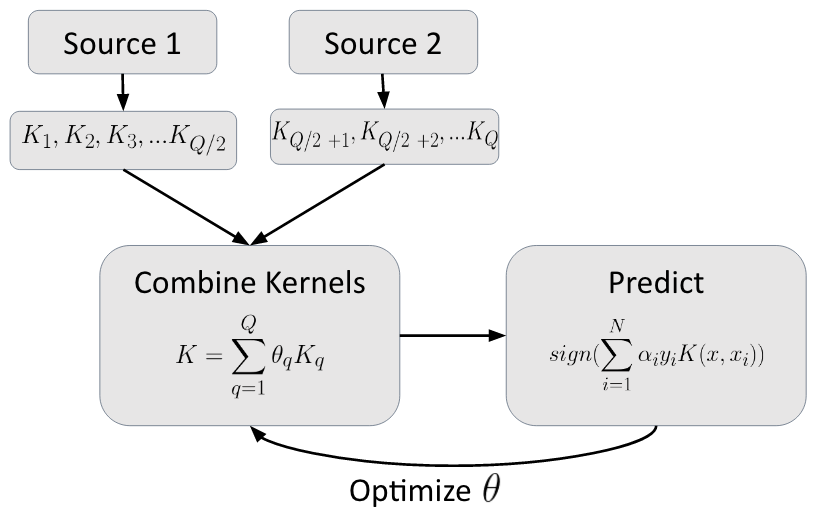
\includegraphics[scale=.4]{implementation_flowchart}
\captionof{figure}{Flow Chart of Our Model}
\end{center}
\end{minipage}



\end{document}
